\section{实证比较}
\subsection{4.1 股票注意力}
\begin{frame}{“更受关注”可以指三种不同结果}
  \strap{4.1\quad 分析单位为股票×月份}
  \begin{tabularx}{\linewidth}{@{}L{.25\linewidth}Y@{}}
    \toprule
    \textbf{经济问题} & \textbf{被解释变量}\\
    \midrule
    多少人研究？ & $A$：研究该股的投资者比例。\\
    共用多少时间？ & $L=\ln(1+\text{合计分钟})$，合计分钟等于人数乘以参与者平均分钟。\\
    内容向哪侧倾斜？ & $D$：价格相关覆盖率减基本面覆盖率。同一户可进入两类。\\
    \bottomrule
  \end{tabularx}
  \smallskip
  {\small
     \textbf{价格组}\quad 价格图、技术分析\par
     \textbf{基本面组}\quad 盈利、分红、其他基本面、分析师、公司网站}
  \refnote{论文 pp.~29–32，Table 4。前1,000大CRSP股票，3,962个股票月份。}
\end{frame}

\begin{frame}{以规模为基准，再比较股票特征}
  \strap{4.1\quad 从单变量基准到扩展规格}
  \[
    Y_{jm}=\alpha+\beta\,z(\ln MC_{jm})
      +\gamma'Z_{jm}+\delta_{\mathrm{FF49}(j)}+\varepsilon_{jm}
  \]
  \begin{columns}[T,onlytextwidth]
    \column{.43\textwidth}
      \shortlabel{仅市值 · 第1列}\par
      多大程度上能用公司规模解释覆盖率？
    \column{.53\textwidth}
      \shortlabel{扩展规格 · 第3、4、6列}\par
      控制规模、股票特征和行业后，比较覆盖、时长与内容差。
  \end{columns}
  \medskip
  {\small $Y\in\{A,L,D\}$。$Z$含新闻、风险、收益及散户活动等变量。\par
  非虚拟解释变量标准化。系数对应增加一个标准差的条件关联。}
  \refnote{据 Table 4（pp.~49–50）写出扩展规格。原表采用滞后两个月的Newey–West标准误。}
\end{frame}

\begin{frame}{规模首先解释有多少人研究}
  \strap{4.1\quad 只用对数市值解释覆盖率}
  \vfill
  \begin{columns}[c,onlytextwidth]
    \column{.31\textwidth}\centering
      \greatnum{1.01\%}\par\small 原文的平均覆盖率
    \column{.36\textwidth}\centering
      {\Large\textcolor{slate}{\(\longrightarrow\)}}\par
      \small 对数市值高1个标准差
    \column{.31\textwidth}\centering
      \greatnum{2.04\%}\par\small 原文的量级示例
  \end{columns}
  \medskip
  {\small\centering \(+1.03\) 个百分点，\(t=14.42\)，\(R^2=0.315\)\par}
  \vfill
  \nextq{覆盖更广时，是否也更偏向价格信息？}
  \refnote{论文 pp.~29–31，Table 4 第1列。\(R^2\) 表示解释的样本变异比例。}
\end{frame}

\begin{frame}{覆盖、时长与内容的方向可以不同}
  \strap{4.1\quad 横读每行，比较同一特征对应的三项结果}
  {\small
  \begin{tabularx}{\linewidth}{@{}Yrrr@{}}
    \toprule
    \textbf{特征} & \textbf{$A$ 覆盖率} & \textbf{$L$ 总时长} & \textbf{$D$ 内容差}\\
     & {\scriptsize 第3列} & {\scriptsize 第4列} & {\scriptsize 第6列}\\
    \midrule
    \(\ln\)市值 & 1.13 {\scriptsize (11.35)} & 0.49 {\scriptsize (15.23)} & 0.03 {\scriptsize (0.61)}\\
    收益波动率 & 0.09 {\scriptsize (2.80)} & 0.10 {\scriptsize (5.35)} & 0.06 {\scriptsize (4.63)}\\
    \textcolor{wine}{\textbf{动量}} & \textcolor{wine}{\(-0.07\) {\scriptsize (\(-2.23\))}} &
        \textcolor{wine}{0.04 {\scriptsize (2.18)}} & \textcolor{wine}{0.05 {\scriptsize (2.33)}}\\
    分析师覆盖数 & 0.11 {\scriptsize (2.06)} & 0.04 {\scriptsize (2.07)} & \(-0.10\) {\scriptsize (\(-2.42\))}\\
    \bottomrule
  \end{tabularx}}
  \finding{动量与覆盖率负相关，与合计研究时长和相对价格覆盖正相关。}
  \refnote{Table 4（pp.~49–50）。$A,D$ 为百分点，$L$ 为对数变换。括号为原表$t$值。3,962个股票月份，包含FF49行业效应。动量窗口为$t-12$至$t-2$月。}
\end{frame}

\subsection{4.2 家庭研究风格}
\begin{frame}{哪些内容会在同一家庭一起出现？}
  \strap{4.2\quad PCA的输入与比较任务}
  \begin{tabularx}{\linewidth}{@{}L{.23\linewidth}Y@{}}
    \toprule
    \textbf{矩阵结构} & \textbf{变量}\\
    \midrule
    一行 & 一个家庭。\\
    13个主题指标 & 月均研究超过2分钟取1，否则取0。\\
    1个连续指标 & 投机标的倾向，用于观察所研究标的与主题配置怎样共同变化。\\
    \bottomrule
  \end{tabularx}
  {\small
  \textbf{主题列}\quad 综合行情、未知新闻、讨论板、盈利、分红、其他基本面、\mbox{分析师}、所有权、公司网站、价格图、技术分析、其他、无法判断。}
  \nextq{先看各类主题是否共同参与，再看内容偏好是否与标的倾向相关。}
  \refnote{论文 p.~35，Table 5（p.~51）。风险统计因参与极少而排除。横截面的完整输入矩阵未公开。}
\end{frame}

\begin{frame}{PC1主要反映跨主题的共同参与}
  \strap{4.2\quad 各主题载荷大多同向，投机标的倾向接近零}
  \centering
  \begin{tikzpicture}[x=7.45cm,y=.51cm]
    \draw[quiet!55] (0,.45)--(0,6.6);
    \foreach \y/\k/\v/\n in {6/{分析师}/.32/0.32,5/{价格图}/.31/0.31,4/{盈利}/.29/0.29,
      3/{其他基本面}/.28/0.28,2/{讨论板}/.16/0.16,1/{投机标的倾向}/.01/0.01}{
        \node[anchor=east,font=\small] at (-.016,\y) {\k};
        \fill[wine] (0,\y-.17) rectangle (\v,\y+.17);
        \node[anchor=west,font=\small,text=wine] at (\v,\y) {\n};
    }
    \node[below,font=\scriptsize] at (0,.42) {0};
    \node[anchor=west,font=\small\bfseries,text=slate] at (.52,4.9) {26.81\%};
    \node[anchor=west,font=\scriptsize,text=slate] at (.52,4.2) {解释变异份额};
  \end{tikzpicture}
  \raggedright
  \finding{高载荷落在不同主题上。PC1描述家庭是否广泛参与各类研究。}
  \refnote{据 Table 5（p.~51）选绘，保留原表符号。}
\end{frame}

\begin{frame}{PC2把内容侧重与标的倾向联系起来}
  \strap{4.2\quad 从正负两侧读这一条方向}
  \centering
  \begin{tikzpicture}[x=7.45cm,y=.45cm]
    \draw[quiet!55] (0,.35)--(0,8.45);
    \foreach \y/\k/\v/\n/\sty/\anch in {8/{讨论板}/.46/+0.46/wine/west,
      7/{投机标的倾向}/.43/+0.43/wine/west,6/{价格图}/.19/+0.19/wine/west,
      5/{分析师}/0/0.00/quiet/west,4/{技术分析}/-.11/\(-0.11\)/slate/east,
      3/{其他基本面}/-.29/\(-0.29\)/slate/east,2/{盈利}/-.34/\(-0.34\)/slate/east,
      1/{分红}/-.47/\(-0.47\)/slate/east}{
        \node[anchor=east,font=\scriptsize] at (-.63,\y) {\k};
        \fill[\sty] (0,\y-.16) rectangle (\v,\y+.16);
        \node[anchor=\anch,font=\scriptsize,text=\sty] at (\v,\y) {\n};
    }
    \node[below,font=\scriptsize] at (0,.32) {0};
  \end{tikzpicture}
  \raggedright
  \finding{PC2解释8.77\%。标的倾向参与了构造，载荷刻画联合共变。}
  \refnote{据 Table 5（p.~51）选绘。符号按原表，可整体翻转。}
\end{frame}

\subsection{4.3 交易时点}
\begin{frame}{同股研究在交易附近迅速累积}
  \begin{columns}[c,onlytextwidth]
    \column{.73\textwidth}
      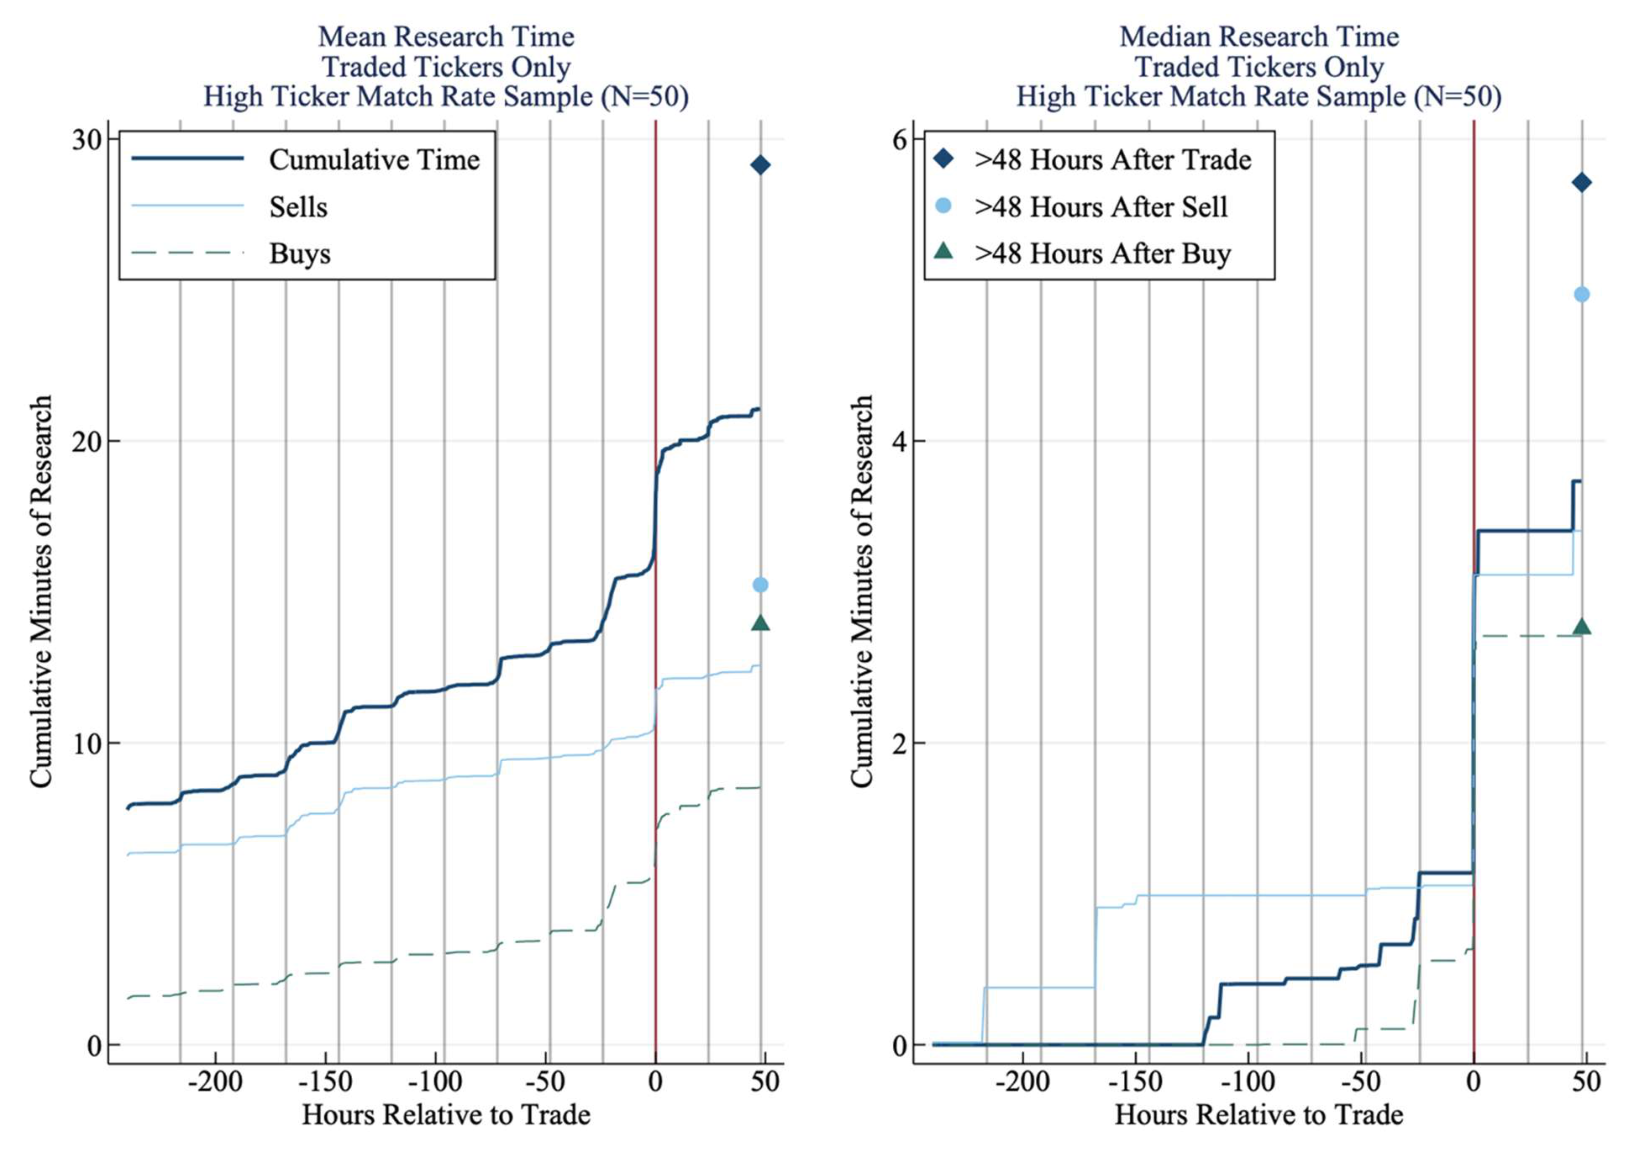
\includegraphics[width=\linewidth,height=5.15cm,keepaspectratio]{trade-timing.png}
    \column{.24\textwidth}
      \small
      \shortlabel{先看右图}\par
      中位数在交易时点附近跳升。
      \medskip\par
      \shortlabel{再看左图}\par
      均值在较早时点已有累积。
  \end{columns}
  \smallskip
  {\small 横轴为相对交易的小时，红线为0。纵轴为累计分钟，两图尺度不同。}
  \refnote{Figure 3（p.~54），50户高匹配样本。左端可含窗口前的累积，右端符号为样本期末总量。}
\end{frame}

\begin{frame}{相同的主题合计，也可以有不同的顺序}
  \strap{4.3\quad 十天内，同一主题只保留第一次出现}
  {\small
  \begin{tabular}{@{}ll@{}}
    原序列 & 价格图 → 盈利 → 分红 → 再看价格图\\
    保留后 & \textcolor{wine}{价格图 → 盈利 → 分红 → END}
  \end{tabular}\par}
  \smallskip
  \begin{columns}[c,onlytextwidth]
    \column{.72\textwidth}
      \begin{tikzpicture}
        \node[inner sep=0] (path) {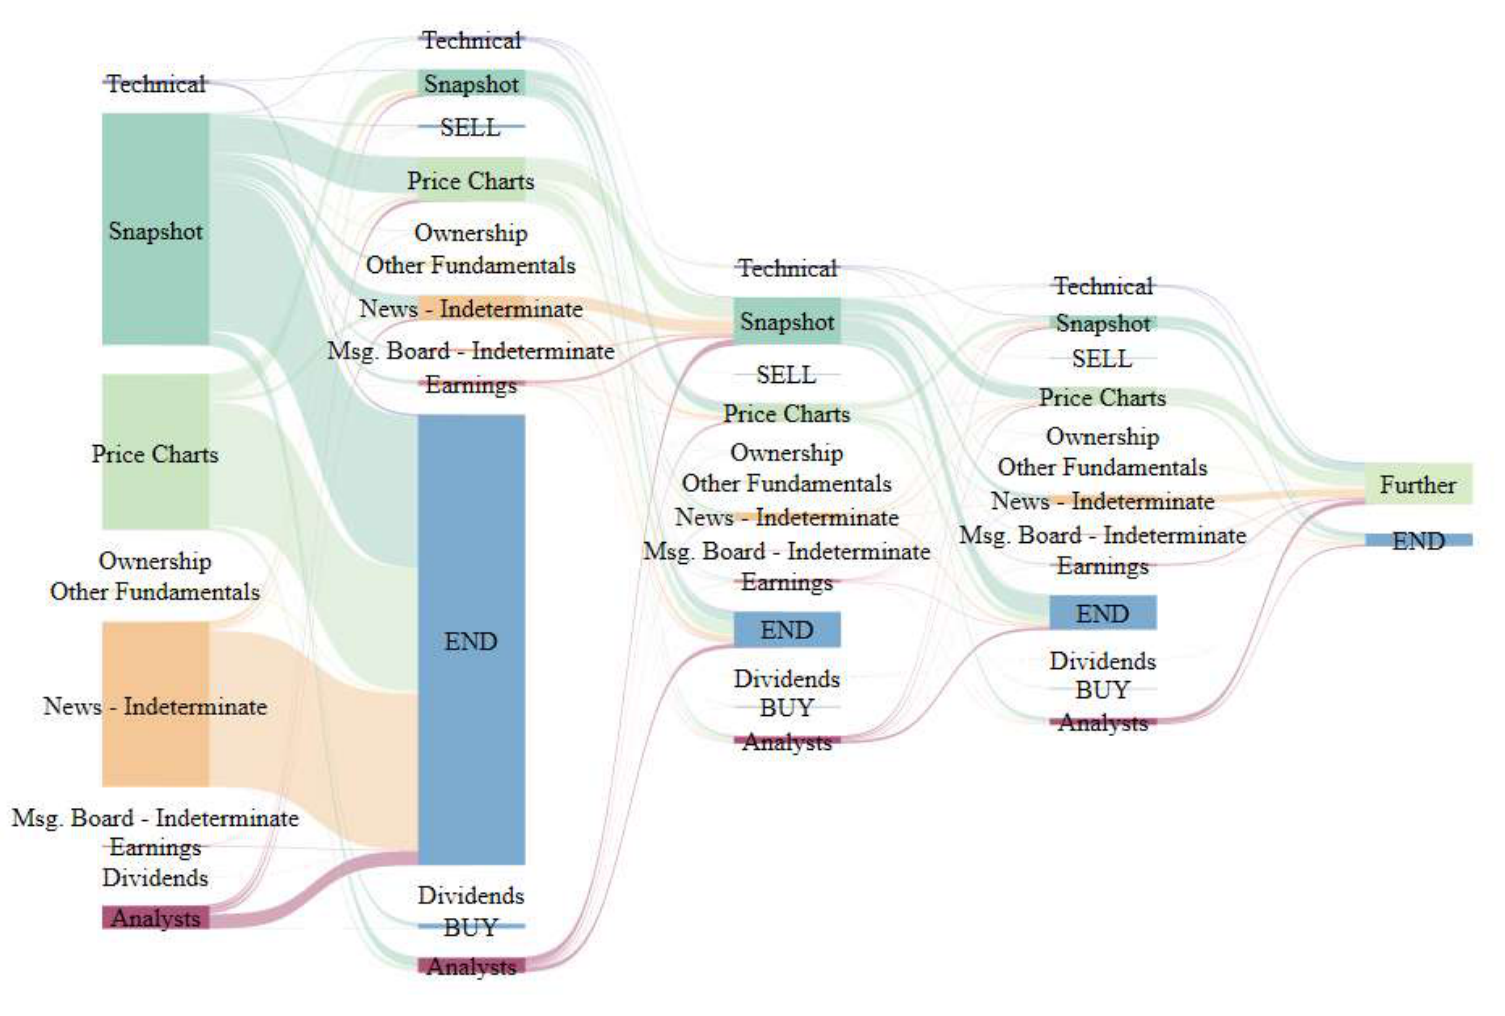
\includegraphics[width=\linewidth,height=4.26cm,keepaspectratio]{research-paths.png}};
        \draw[wine,thick,rounded corners=1pt]
           ($(path.south west)!.065!(path.south east)+(0,2.70)$) rectangle
           ($(path.south west)!.15!(path.south east)+(0,3.76)$);
        \draw[slate,thick,rounded corners=1pt]
           ($(path.south west)!.27!(path.south east)+(0,.63)$) rectangle
           ($(path.south west)!.36!(path.south east)+(0,2.56)$);
      \end{tikzpicture}
    \column{.25\textwidth}
      \small
      \shortlabel{读左边两列}\par
      酒红框：综合行情是常见入口。\par
      蓝框：第一步之后结束。
  \end{columns}
  \refnote{Figure 4（p.~55），484户、16,930个融合窗口。只留主题首次出现，线宽表示窗口数。}
\end{frame}

\begin{frame}{回看买卖之前，粗主题次序相近}
  \strap{4.3\quad 从交易端向左回看前一组主题}
  \begin{columns}[c,onlytextwidth]
    \column{.48\textwidth}\centering\shortlabel{买入前}\par
    \column{.48\textwidth}\centering\shortlabel{卖出前}\par
  \end{columns}
  \centering
  \begin{tikzpicture}
    \node[inner sep=0] (paths)
      {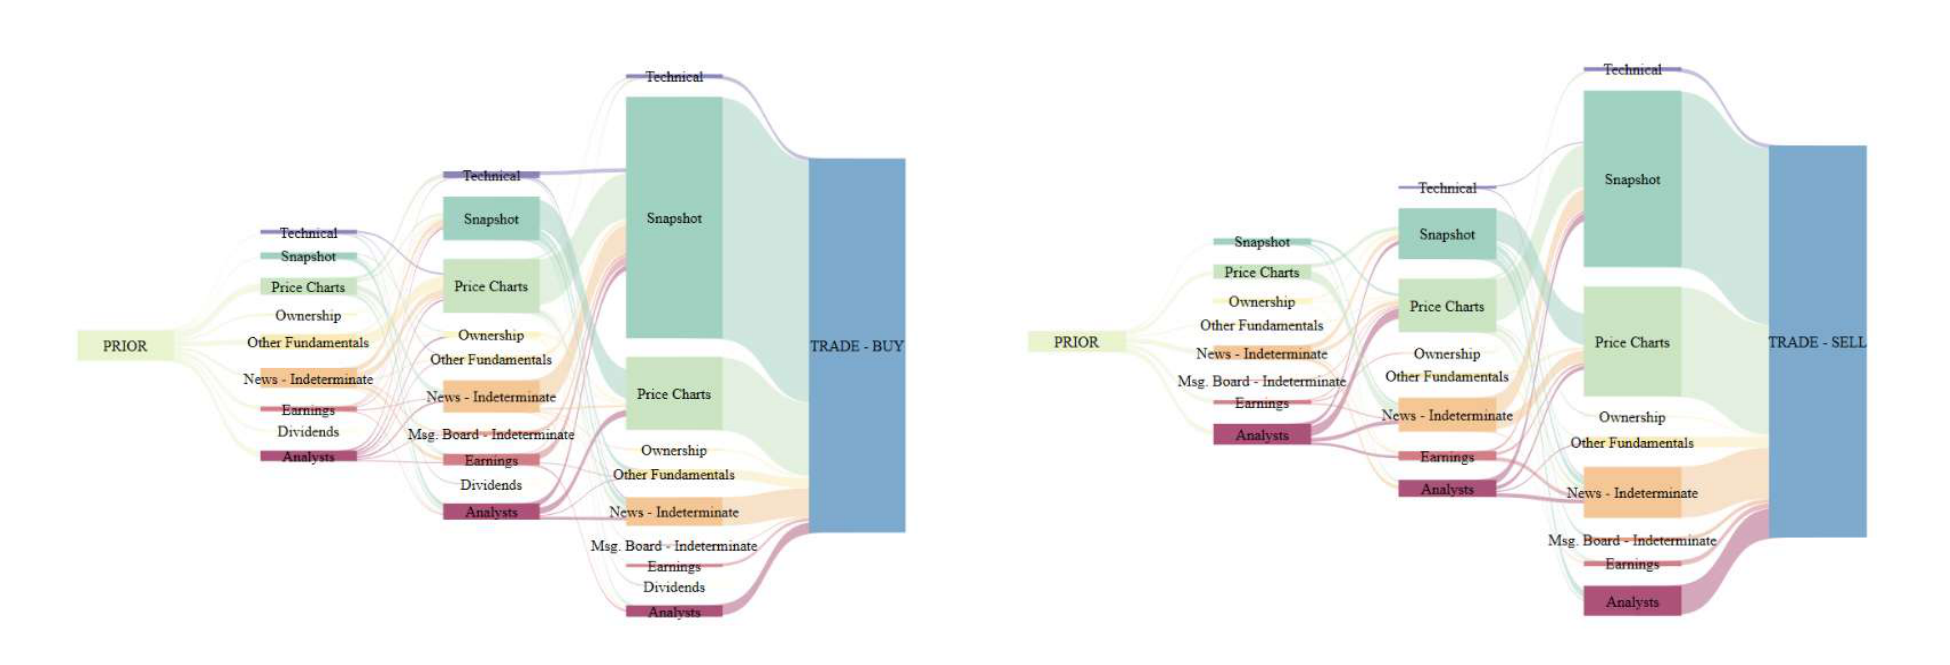
\includegraphics[width=.99\linewidth,height=4.35cm,keepaspectratio]{paths-by-direction.png}};
    \draw[wine,thick,rounded corners=1pt]
       ($(paths.south west)!.316!(paths.south east)+(0,1.39)$) rectangle
       ($(paths.south west)!.377!(paths.south east)+(0,3.37)$);
    \draw[wine,thick,rounded corners=1pt]
       ($(paths.south west)!.807!(paths.south east)+(0,1.51)$) rectangle
       ($(paths.south west)!.868!(paths.south east)+(0,3.41)$);
  \end{tikzpicture}\par
  \raggedright
  \finding{两侧临近交易处都突出综合行情和价格图。解释买卖方向还需要具体信号、先验或持仓。}
  \refnote{Figure 5 Panels A–B（p.~56）。线宽按窗口数，比较面板内的主题顺序。}
\end{frame}
